% Template: LaTeX file for ICMC 2011 papers, with hyper-references
%
% derived from the DAFx-06 templates
% derived from the ICMC 2009 templates by Steve Beck
% and then derived from the ICMC 2010 template
% 1) Please compile using latex or pdflatex.
% 2) Please use figures in vectorial format (.pdf); .png or .jpg are working otherwise 
% 3) Please use the "papertitle" and "pdfauthor" commands defined below

%------------------------------------------------------------------------------------------
\documentclass[twoside,10pt,a4paper]{article}
\usepackage{icmc2011,amssymb,amsmath} 
\usepackage{listings}

\lstset{
language=Python,
basicstyle=\footnotesize,
numbers=left,
numberstyle=\tiny,
columns=fullflexible,
showstringspaces=false
}

%\setcounter{page}{1}

\usepackage{mathptmx} 

%____________________________________________________________
%  !  !  !  !  !  !  !  !  !  !  !  ! user defined variables  !  !  !  !  !  !  !  !  !  !  !  !  !  !
%==== set the title ====
\def\papertitle{The Integra Framework for rapid modular audio application development}
%\def\papertitle{}	%-- should be empty for the submission anyway!

%==== 1st submission: author name and affiliation are empty for anonymous submission ====
\def\paperauthorA{Jamie Bullock} 
\def\paperauthorB{Henrik Frisk} 

\twoaffiliations{\paperauthorA, }{Birmingham Conservatoire\\ Birmingham, UK \\ {\tt\href{mailto:jamie.bullock@bcu.ac.uk}{jamie.bullock@bcu.ac.uk}}}
{\paperauthorB}{Lund University\\ Malm\"{o}, Sweden \\ {\tt\href{mailto:mail@henrikfrisk.com}{mail@henrikfrisk.com}}}


%==== final submission: author name and affiliation ====
%---- uncomment 1 to 4 lines, for 1 to 4 authors
%\def\paperauthorA{First Author}
%\def\paperauthorB{Second Author}
%\def\paperauthorC{Third Author}%
%\def\paperauthorD{Fourth Author}

%%---- set correspnding affiliation data for...
%%-- 1 author
%\affiliation{\paperauthorA}
%  {School\\ Department, City, Country \\ {\tt \href{mailto:email@domain.icmc}{email@domain.icmc}}}

%%-- 2 authors with same affiliation
%\affiliation{\paperauthorA, \paperauthorB}
%  {School\\ Department, City, Country \\ {\tt \href{mailto:email@domain.icmc}{email@domain.icmc}}}

%-- 2 authors with different affiliations
%\twoaffiliations{\paperauthorA}{School\\ Department}
%  {\paperauthorB}{Company\\ Address}

%%-- 3 authors with different affiliations
%\threeaffiliations{\paperauthorA}{School A\\ Department X}
%  {\paperauthorB}{Company\\ Address}
%  {\paperauthorC}{School B\\ Department Y}

%%-- 4 authors with different affiliations
%\fouraffiliations{\paperauthorA}{School A\\ Department X}
%  {\paperauthorB}{Company\\ Address}
%  {\paperauthorC}{School B\\ Department Y}
%  {\paperauthorD}{School C\\ Department Z}

%  ^  ^  ^  ^  ^  ^  ^  ^  ^  ^ user defined variables  ^  ^  ^  ^  ^  ^  ^  ^  ^  ^  ^  ^ 
%------------------------------------------------------------------------------------------

%%-- if using .ps or .eps figure files, they will be converted on the fly
%%-- RMK: for faster LaTeX runs, use it only once after adding new \includegraphics[]{} cmds
%\usepackage{epstopdf}	 

%---- the hyperref package must be last to properly work
\usepackage[pdftex,
       pdftitle={\papertitle},
	pdfauthor={\paperauthorA},
	colorlinks=false,bookmarksnumbered,pdfstartview=XYZ]{hyperref}
%\pdfcompresslevel=9
\usepackage[pdftex]{graphicx}	% for compatible graphics with hyperref
\usepackage[figure,table]{hypcap}	% corrects the hyper-anchor of figures/tables
\usepackage{verbatim}
\title{\papertitle}

%------------------------------------------------------------------------------------------
\begin{document}

\DeclareGraphicsExtensions{.png,.jpg,.pdf} % used graphic file format for pdflatex
    
\maketitle

\begin{abstract}
In this paper, we present the Integra Framework as a platform for the rapid and sustainable development of audio processing software. The framework provides a simple, robust API for managing graphs of connected modules, querying state and state saving as well as a dynamic OSC interface for real-time control. Additionally, the framework comes with extensive documentation and library of core modules for performing common tasks. This allows developers to create working, usable applications within days and to focus on research and development of novel user interfaces. As evidence of the framework's benefits, we present integra Live, a full-featured application for live electronics, developed in 9 months. 
\end{abstract}

\section{Introduction}\label{sec:introduction}


The research and development process for the Integra \linebreak Framework was conducted under the auspices of Integra a 3 year EU-funded project led by Birmingham Conservatoire, following another 3-year EU-funded project, ``Integra, A European Composition and Performance Environment for Sharing Live Music Technologies'', both supported by the Culture programme of the European Commission. One of the main goals of Integra is to develop a new software environment for the composition and performance of live electronic music \cite{Bullock:01}. In the first 3-years of the project the focus was largely on creating a shared library (libIntegra) that would enable the separation of audio connection graphs and parameter state, from any specific DSP host\cite{Bullock:02}. In `Integra 2', the focus shifted to user interface development, and libIntegra became the core of the Integra Framework, which was developed in parallel with the Integra Live GUI\cite{Bullock:01}.

At the beginning of Integra 2, in 2009 the project had produced a prototype GUI developed in Max and Java\-script\cite{Bullock:01}, and a proof-of-concept abstraction layer in the form of libIntegra. The challenge was then to develop a fully-fledged application that could be used in public concerts for the live electronics elements of the Integra 2 commissioned composers and performers\footnote{\href{http://www.integralive.org}{http://www.integralive.org}}. The software needed to be simple enough to be used by composers with little previous experience in live electronics, and still have the functionality to support the Integra 2 migration programme, which includes porting works by Grisey, Saariaho, Hurel and others to the software. 

The decision was therefore made to expand our existing work on libIntegra into a framework that would support the needs of the Integra GUI as it developed. So whilst we followed an Agile, user-centred methodology in the development of Integra Live, a similar iterative methodology was adopted enabling the framework to support the requrements of the GUI. We believe this reciprocation between GUI and framework has led to a more robust framework, better suited to the demands of practical applications.

\section{Existing Work}\label{sec:existing_work}

The Integra Framework largely derives from libIntegra, a lightweight library for software-independent multimedia module description and storage\cite{Bullock:03}. libIntegra includes facilities for the separation of DSP processing, processing graph storage and management, and state saving. It takes inspiration from 4MPS, including the separation of data and processing\cite{Amatriain:00}, as well as the Jamoma project, which seeks to address common concerns\cite{Place:02}. However libIntegra places a stronger emphasis on creating a client-server model for user interface development, where the UI acts as a client to the libIntegra server. The functionality of libIntegra is discussed extensively in\cite{Bullock:03}, \cite{Bullock:02} and \cite{Bullock:00}, and only elementes of libIntegra that are new or changed will be discussed in later sections.

Other subsequent frameworks that provide similar functionality include the Jamoma Audio Graph and Jamoma DSP Frameworks, which like libIntegra make a separation between audio `UGen' hosting and the creation and editing of graph structures used to represent UGens and their connections\cite{Place:00}. Jamoma was considered as a possible alternative to libIntegra as a platform for the Integra GUI, but at the time of development in 2009, the Jamoma frameworks weren't sufficiently developed. The Integra Framework was therefore developed as a parallel effort.


\section{The Framework}\label{sec:the_framework}

In addition to the core functionality provided by libIntegra, the Integra Framework provides a set of core classes. These are classes that are flagged as `core' in the Integra database, and as such they get distributed with the framework and can be made available in any client using the framework.

\subsection{Base Classes}\label{subsec:base_classes}

A selection of the core base classes are shown in figure~\ref{fig:class_diagram}. Classes shown in italics are `abstract' and can't be instantiated in libIntegra. Classes under the Module branch (hereafter referred to as `modules'), have additional metadata associated with their attributes as well as their type. This metadata includes attribute mimima and maxima, unit, and scale. Functionality for enumerations is provided \linebreak through a `legal values' field in the attribute definition. Like the other metadata fields described here this provides information to clients using the framework. It is up to the client to respect the legal values enumeration for any given attribute, and the behaviour for non-legal values is undefined. Additionally, the attribute definition contains a `value labels' list that can be used to suggest potential labels to client or add semantic meaning. The following table shows a fictious PentatonicFilter module whose frequency maps to a pentatonic scale. The advantage of deferring to the client to adhere to the metadata in the module definition is that we can provide a range of different modules with a common base class simply by changing the {\it interface} in the sub-classes.

\begin{figure}[htbp]
\centerline{\framebox{
	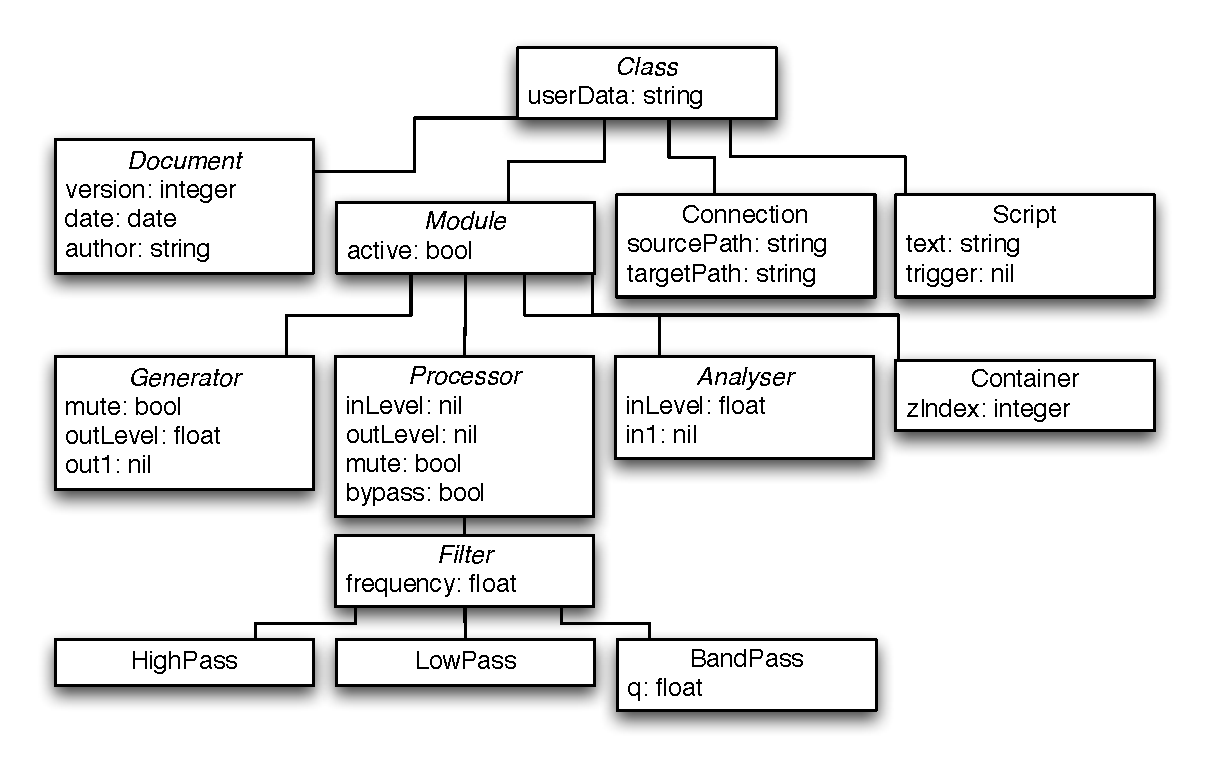
\includegraphics[width=1.0\columnwidth]{class_diagram}}}
\caption{Selection of base classes from the Integra Framework}
\label{fig:class_diagram}
\end{figure}

The live database with a fully browsable list of classes and their attributes can be found at http://db.integralive.org.

\begin{table}[htbp]
\begin{center}
\begin{tabular}{|l|l|}
\hline
field & value \\
\hline
name  & frequency \\
type & float \\
unit & Hertz \\
control class & slider \\
control attribute & value \\
allowed values 1 & 440 \\
allowed values 2 & 493.8 \\
allowed values 3 & 554.3 \\
allowed values 4 & 659.2 \\
allowed values 5 & 739.9 \\
\hline
\end{tabular}
\end{center}
\caption{Attribute definition for a frequency attribute that locks to a pentatonic scale}
\label{tab:example}
\end{table}


\subsection{Modules}

Modules are classes that are defined under the Module base class, and make up the majority of classes in the hierarchy. Modules are implemented in a module host, which libIntegra communicates with via a host-specific bridge\cite{Bullock:03}. Currently the framework only supports Pure Data as a host, but support for Max is also underway. 

The framework comes bundled with a substantial and growing collection of core modules designed to be general enough to have immediate musical application, but specific enough that large portions of functionality aren't duplicated between classes. The available range of modules has so far been determined largely by the requrements of Integra 2 migrations and commissions\footnote{\href{http://www.integralive.org}{http://www.integralive.org}}.

A Pd module development SDK is provided as part of the framework so that users and developers can create their own module implementations. This SDK makes it easy-as-possible to create new modules by supplying customisable templates. In the majority of cases it is enough to take an existing module implementation and simply replace the DSP `guts' and attribute names so that the interface corresponds to that defined in the database.

\subsection{System classes}

Classes may optionally be flagged `system' in their definition in the Integra database. System classes are fundamental parts of the framework, and may be implemented partially or entirely in libIntegra itself. Examples of system classes include Script, which provides access to the framework scripting functionality implemented in libIntegra, and Connection, which is implemented in libIntegra for asynchronous (message passing) connections, and in the module host for synchronous connections. A similar separation of synchronous and asynchronous processing is made in other frameworks such as Jamoma\cite{Place:00} and CLAM\cite{Amatriain:00}.

\subsection{Controls}

Module attributes can optionally be assigned a `control class', `control attribute' and `control group'. These fields act as hints to the client as to how the attribute should be controlled. Control classes aren't part of the main class hierarchy, but instead defined in a lookup table. As such the range available classes is constantly expanding. Single-attribute controls include Knob, Slider, Checkbox, RadioGroup, VuMeter, Trigger and NumberBox. Multi-attribute controls include XYScratchPad, XYPanPad, RoomShape and RangeSlider. Each control class has a description and a reference implementation in Adobe Flex\footnote{\href{http://www.adobe.com/products/flex/}{http://www.adobe.com/products/flex/}}. Multi-attribute controls are associated with attributes using the control group field in the database.

A simple XML-based format is provided for specifying control layouts. Clients can optionally use the frame\-work-supplied module control layouts for laying out multiple controls. An example of such a file is shown in listing~\ref{layout_xml} below, with the corresponding control layout shown in figure~\ref{fig:control_layout}. Application developers can make use of the Flex reference implementations if their client GUI development framework permits, or devise their own control implementations accordingly.

\begin{lstlisting}[label=layout_xml,caption=Module control layout XML]
<controls>
<control id="active" x="20" y="10" width="70" height="85"/>
<control id="bypass" x="20" y="105" width="70" height="85"/>
<control id="inLevel" x="100" y="10" width="50" height="180"/>
<control id="outLevel" x="160" y="10" width="50" height="180"/>
<control id="mix" x="220" y="10" width="190" height="180"/>
<control id="posXY" x="420" y="10" width="180" height="180"/>
</controls>
\end{lstlisting}

\begin{figure}[htbp]
\centerline{\framebox{
	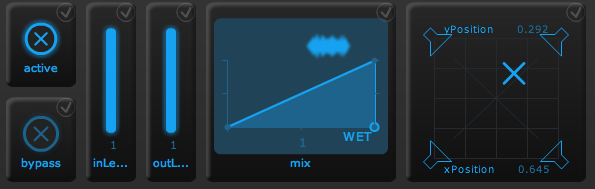
\includegraphics[width=1.0\columnwidth]{controls}}}
\caption{Controls laid out according to XML layout file}
\label{fig:control_layout}
\end{figure}

\section{Instances and connections}

Once a module has a definition (created in the Integra database) and an implementation (in Pd), it can be instantiated at runtime. libIntegra builds a dynamic representation of all module definitions by introspecting the database (or a local copy of it), and uses this to supply information to clients via XMLRPC (cf. section~\ref{sec:xmlrpc}). Clients can then request module creation within a given parent node up to an arbitrary level of nesting. An abstract Container class is provided for nodes whose only purpose is to logically group modules, but nesting can also be useful for creating one-to-one or one-to-many associations between instances. Examples include the Envelope class, which can contain many ControlPoint nodes, and the Tx816 module, which contains 8 TF1 nodes.

Attributes can be connected using instances of the Connection class. \verb!Connection.sourcePath! and \linebreak\verb!Connection.targetPath! can be set independently and when both attributes have a valid value a connection will be made. Attributes can only be connected to attributes of sibiling nodes or children of sibling nodes, that is connections can't be made outside of a node's enclosing node. This makes it possible to re-parent nodes without breaking referential integrity. libIntegra allows multiple Connection instances to refer to the same attribute allowing for one-to-many or many-to-one 'fanning' connections. In the case of audio connections many-to-one connection results in implicit summing of synchronous audio blocks, for messaging connections, messages are simply processed in arrival order.

\section{OSC API}

When a class is instantiated using libIntegra, it becomes immediately addressable via open sound control. libIntegra runs as an OSC server on a UDP port determined at startup. Module instances are addressable using their node path expressed as an OSC address string, for example:
{\small \begin{verbatim}Project1.Envelope1.ControlPoint1.value\end{verbatim} }
\begin{flushleft}
Would be addressed using:
\end{flushleft}
{\small {\begin{verbatim}/Project1/Envelope1/ControlPoint1/value\end{verbatim}}

OSC supported type codes correspond to the Integra data types defined in \cite{Bullock:03}, currently `f', `i', 's', `b' and `n'. If a node gets renamed, deleted or moved within the node graph, the OSC namespace is updated accordingly.

\section{XMLRPC API}\label{sec:xmlrpc}

The libIntegra XMLRPC API provides access to the full functionality of the library including facilities for introspecting available classes and their attributes through a simple query API. XMLRPC was chosen for its combination of bi-directional messaging (something OSC lacks), and simplicity compared to other XML-based protoctols such as SOAP. It is possible to develop XMLRPC libIntegra clients easily in a range of languages with XMLRPC support. Using languages that provide an interactive interpreter, it's even possible to `live code' with the Integra Framework. A simple example is shown in listing~\ref{livecode_py}.

\begin{lstlisting}[label=livecode_py,caption=XMLRPC API from Python]
import xmlrpclib

p = xmlrpc.ServerProxy('http://localhost:8000')

p.new(`AudioIn', `AudioIn1', None)
p.new(`AudioOut'', `AudioOut1', None)
p.new(`Connection', `Connection1' , None)
p.set(`Connection1', `sourcePath', `AudioIn1.out1')
p.set(`Connection1', `targetPath', `AudioOut1.in1')

\end{lstlisting}


\subsection{Scripting Interface}

In addition to external access via XMLRPC libIntegra supports internal scripting using the Script class. Unlike signal processing modules, the Script class is implemented in the library. It provides a layer on top of the Lua scripting language, which was chosen for its simple syntax, simplicity of compilation and portability. Integra Lua script provides a somewhat leaner syntax than that shown above. For example, using the Integra CLI or the Script class, we can rewrite the above Python code in Integra script as follows:

\begin{lstlisting}
AudioIn1 = new(`AudioIn')
AudioOut1 = new(`AudioOut')
AudioIn1.out1 = AudioOut1.in1
\end{lstlisting}

\section{Local Storage}

The Integra Framework provides an extensible XML-based format, IXD (Integra eXtensible Data), which can be used for storing graphs of class instances and instance attribute state\cite{Bullock:02}. libIntegra is capable of reading and writing IXD, as well as validating against the Integra collection XML Schema. When saving, a parent node is specified as a save-from point, and when loading a node is specified for loading under. This allows for arbitrary import and export of parts of the node graph including export of individual instances. This enables clients to build preset save and load functionality on top of libIntegra's API.

\subsection{Online Storage}
In addition to loading the IXD files in IntegraLive, users may also upload their projects to the Integra Documentation Browser, a web application for documenting and sharing of primarily IXD files. The documentation browser, however, may also be used for more general work documentation and annotated scores. When uploaded, the user may create views of the uploaded IXD showing only selected elements of the project file, and it is furthermore possible to add documentation to these, or any other sections of the project file. This can for example be instructions on how to perform a particular live electronic part. The documentation browser may also be used by the composer to prepare material to be included with the score by exporting a view of the project file to PDF. Written in XQuery, a functional programming language with strong typing features, the documentation browser uses the eXist native XML database as its backend.

\section{Framework In Use}

The framework has now moved beyond the proof-of-concept stage outlined in\cite{Bullock:02}, and serves as the basis for the Integra Live software for live electronics composition and performance, currently in public beta\footnote{\href{http://download.integralive.org}{http://download.integralive.org}}. Packaging modular audio processing, graph management, introspection and state saving into an easy-to-use framework enabled the development of the Integra Live GUI in only 9 months. The GUI is written in Adobe Flex, and acts as a `dumb client' to the libIntegra XMLRPC server, populating its module list and building control names and ranges through introspection. In Integra Live, `system' classes are provided transparently, for example the Script class appears in the UI, not as a draggable module, but as a `tab' that is associated with the currently selected 'block' or 'track'. In addition to the Integra CLI and Integra Live GUI, the framework is also used as the basis of a growing number of other audio apps including Sonar2D, an audio feature-driven application.

\section{Conclusions}

In this paper we have outlined a full-featured and robust framework for the rapid development of modular audio software. The framework has a variety of applications including live coding via the XMLRPC API, or using the Integra script provided with the command-line interface. It also makes an excellent rapid development platform, and allows developers to focus on user interface design without worrying about low-level DSP functionality, file I/O and graph management. The framework is also extensible using the Pd module development SDK, with which developers can quickly create new processing modules or modify existing ones.

\bibliographystyle{IEEEtranS}
\bibliography{template} % requires file template.bib
\end{document}

%
%This is the template file for the proceedings of the 9$^{th}$ International Conference on Digital Audio Effects (DAFx-06). 
%This template has been generated from WASPAA'99 templates and aims at producing conference proceedings in electronic form. 
%The format is essentially the one used for ICASSP conferences.

%Please use either this \LaTeX{} or the accompanying Word formats when preparing your submission. 
%The templates are available in electronic form at the website:
%\\ \href{http://www.dafx.ca}{http://www.dafx.ca}. Thanks!

%

%
%This template can be found on the conference website.

%\subsection{Figures} 
%All figures should be centered on the column (or page, if the figure spans both columns). 
%Figure captions (in italic) should follow each figure and have the format given in Figure \ref{fft_plot}.
%\begin{figure}[ht]
%\centerline{\includegraphics[scale=0.8]{fft_plot2}}
%\caption{{\it Sinusoid in time and frequency domain.}}  
%\label{fft_plot}
%\end{figure}
%Figures must be vectorial (no screen copy, no bitmap, etc). For example when using \texttt{Matlab}, export using either Postscript or PDF format. Also, in order to provide a better readibility, figure text font size should be at list identical to footnote font size. To do so using \texttt{Matlab}, use the \texttt{subplot} command before plotting.

%\subsection{Tables} 
%As for figures, all tables should be centered on the column (or page, if the table spans both columns). 
%Table captions should be in italic, follow each table and have the format given in Table \ref{tab:example}.

%\begin{table}[htdp]
%  \begin{center}
%    \begin{tabular}{|c|c|}\hline
%    	angle ($\theta$, rad) & $\sin \theta$ \\\hline
%	$\frac{\pi}{2}$ & 1 \\
%	$\pi$ & 0 \\
%	$\frac{3\pi}{2}$ & -1 \\
%	$2\pi$ & 0 \\\hline
%    \end{tabular}
%  \end{center}
%  \label{tab:example}
%  \caption{{\it Basic trigonometric values.}}
%\end{table}%

%\subsection{Equations}
%Equations should be placed on separate lines and numbered:

%\begin{equation}
%X(e^{j\Omega})=\sum_{n=0}^{N-1}x(n)e^{-j\Omega n}
%\label{eq1}
%\end{equation}
%where the sequence $x(n)$ in equation (\ref{eq1}) is a windowed frame:
%\begin{equation}
%x(n)=s(n)\cdot w(n)
%\label{eq2}
%\end{equation}
%with a window function $w(n)$.

%\subsection{Page Numbers}
%Page numbers will be added to the document electronically, so {\em please leave the numbering as is},
%that is, the first page will start at page DAFX-1 and the last page, at most, will have to be DAFX-6
%for the submission of papers for an oral presentation or DAFX-4 in the case of a poster presentation.

%\subsection{References}
%The references will be numbered in order of appearance \cite{Mitra:Kaiser:1993:DSP:handbook}, \cite{Haykin:1991:adaptive:filter}, \cite{Moorer:2000:AES:audio:millenium} and \cite{Arfib:1998:DAFx}. Please avoid listing references that do not appear in the text (we did the opposite in this template).

%\subsubsection{Reference Format}
%The reference format is the standard IEEE one. We recommend to use BibTeX to create the reference list.

%\section{Conclusions}
%This template can be found on the conference website. 
%If you wish to include two authors' affiliations please use the companion LaTeX template tmpl\_la2\_href. 
%Please, submit full-length papers (max.~6 pages for oral presentation and max.~4 pages for posters).
% 
%Submission is fully electronic and automated through the Conference Web Submission System. 
%DO NOT send us papers directly by e-mail. 

%\section{Acknowledgements}
%Many thanks to the great number of anonymous reviewers!

%%\newpage
%\nocite{*}
%\bibliographystyle{IEEEbib}
%\bibliography{template} % requires file template.bib

%\end{document}
